\section{Risultati}
La validazione dei modelli appena discussi è stata effettuata confrontando i
risultati della simulazione con le stime dedotte dall'analisi, valutando quattro
possibili scenari contraddistinti dal valore che assume il parametro $S$.

Ognuno di questi scenari è stato simulato facendo processare al programma lo
stesso numero di job affinché le statistiche globali del sistema possano
essere confrontate. Tale numero è stato stabilito in base alle metriche che
andavano valutate ed al numero di job che le riguardava.

Lo scenario con valore di soglia $S=5$, è quello in cui soltanto circa il $2\%$
dei job di classe 2 è processato nel cloudlet e di questi circa il $90\%$
vengono interrotti, ne risulta, quindi che in relazione al numero totale dei job
che transitano nel sistema, solamente lo $0.14\%$ sono job di classe 2
processati con successo nel cloudlet e l'$1.37\%$ sono job interrotti. In
definitiva, al fine di avere una dimensione dei batch soddisfacente per il
calcolo delle relative metriche, è stato scelto un numero totale di job pari a
$500000$. In questo modo si ottiene un numero di job di classe 2 processati con
successo nel cloudlet pari a circa $700$ e un numero di job interrotti pari a
circa $6850$, ciò significa che per un valore $k=64$ corrispondente al numero
di batch, si ottengono batch di dimensione $10$ e $107$ rispettivamente, che
sono sufficienti a determinare intervalli di confidenza, seppur con un ampio
margine di errore.

Quello appena descritto è il peggior scenario possibile, in cui si registra il
minor numero di job per una determinata metrica, gli altri scenari vengono
quindi simulati tutti con un numero totale di job pari a $500000$, e a seconda
del numero di job che verranno processati nei vari nodi e della loro tipologia,
sono risultati intervalli di confidenza più o meno precisi.

Purtroppo è risultato impossibile determinare risultati attendibili per i job
di classe 1 che vengono processati nel cloud, poiché il loro numero è, per ogni
scenario, talmente esiguo, che per avere un batch di dimensione 10 sarebbero
necessari almeno 3 milioni di job in tutto. Tuttavia, con un numero di
$500000$ job totali, si ottengono delle statistiche globali molto attendibili,
infatti, ad esempio per il tempo medio di risposta del sistema, si ottiene 
una dimensione del batch pari a $\lfloor\frac{500000}{64}\rfloor = 7812$.

Per ogni statistica vengono presentati grafici e tabelle, in cui vengono
confrontati i risulatati osservati in 10 repliche della simulazione con la
relativa stima del modello analitico, inoltre nelle tabelle viene anche indicato
l'errore massimo che è stato commesso, corrispondente al massimo delle distanze 
tra la stima e l'estremo più lontano di ogni intervallo di confidenza.
%
%
%%%%%%%%%%%%%%%%%%%%%%%%%%%%%%%%%%%%%%%%%%%%%%%%%%%%%%%%%%%%%%%%%%%%%%%%%%%%%%%%
%%%%%%%%%%%%%%%%%%%%%%%%%%%%%%%%%%%%%%%%%%%%%%%%%%%%%%%%%%%%%%%%%%%%%%%%%%%%%%%%
\subsection{Scenario 1: $\mathbf{S=N=20}$}
%%%%%%%%%%%%%%%%%%%%%%%%%%%%%%%%%%%%%%%%%%%%%%%%%%%%%%%%%%%%%%%%%%%%%%%%%%%%%%%%
\subsubsection{Tempi di risposta: Cloudlet}
%
\begin{figure}[!h]
\centering
%
\begin{subfigure}[t]{0.49\textwidth}
\includegraphics[width=\textwidth]{figures/simul/20_500K_s1clet}
\caption{classe 1}
\label{20_s1clet}
\end{subfigure}
%
\begin{subfigure}[t]{0.49\textwidth}
\includegraphics[width=\textwidth]{figures/simul/20_500K_s2clet}
\caption{classe 2}
\label{20_s2clet}
\end{subfigure}
%
\begin{subfigure}[t]{0.5\textwidth}
\includegraphics[width=\textwidth]{figures/simul/20_500K_sclet}
\caption{globale}
\label{20_sclet}
\end{subfigure}
%
\caption{tempo di risposta medio cloudlet per $S = 20$}
\end{figure}
%
\begin{table}[!h]
\begin{tabular}{c|r@{.}l|r@{.}l|r@{.}l}
& \multicolumn{2}{|c|}{$S_1^{clet}$}
& \multicolumn{2}{|c|}{$S_2^{clet}$}
& \multicolumn{2}{|c}{$S_{clet}$} 
\\          
\hline
R1      & $2$&$2231 \pm 0.0105$ & $2$&$4074 \pm 0.0153$ & $2$&$2922 \pm 0.0067$ \\
R2      & $2$&$2129 \pm 0.0103$ & $2$&$4115 \pm 0.0172$ & $2$&$2885 \pm 0.0082$ \\
R3      & $2$&$2262 \pm 0.0096$ & $2$&$3949 \pm 0.0164$ & $2$&$2896 \pm 0.0081$ \\
R4      & $2$&$2244 \pm 0.0105$ & $2$&$4221 \pm 0.0175$ & $2$&$2996 \pm 0.0073$ \\
R5      & $2$&$2230 \pm 0.0107$ & $2$&$4125 \pm 0.0172$ & $2$&$2942 \pm 0.0072$ \\
R6      & $2$&$2149 \pm 0.0113$ & $2$&$3891 \pm 0.0148$ & $2$&$2811 \pm 0.0079$ \\
R7      & $2$&$2250 \pm 0.0106$ & $2$&$3929 \pm 0.0173$ & $2$&$2885 \pm 0.0074$ \\
R8      & $2$&$2236 \pm 0.0094$ & $2$&$3962 \pm 0.0168$ & $2$&$2885 \pm 0.0071$ \\
R9      & $2$&$2183 \pm 0.0104$ & $2$&$4046 \pm 0.0167$ & $2$&$2887 \pm 0.0079$ \\
R10     & $2$&$2191 \pm 0.0095$ & $2$&$4107 \pm 0.0168$ & $2$&$2918 \pm 0.0066$ \\
STIMA   & $2$&$2222$            & $2$&$3904$            & $2$&$2884$            \\
MAX ERR & $0$&$0136 \ (0.6\%)$  & $0$&$0492 \ (2.0\%)$  & $0$&$0185 \ (0.8\%)$    
\end{tabular}
\centering
\caption{Confronto tempi risposta cloudlet per $S=20$}
\label{tab:20_sclet}
\end{table}

%%%%%%%%%%%%%%%%%%%%%%%%%%%%%%%%%%%%%%%%%%%%%%%%%%%%%%%%%%%%%%%%%%%%%%%%%%%%%%%%
\subsubsection{Tempi di risposta: Cloud}
%
\begin{figure}[!h]
\centering
%
\begin{subfigure}[t]{0.49\textwidth}
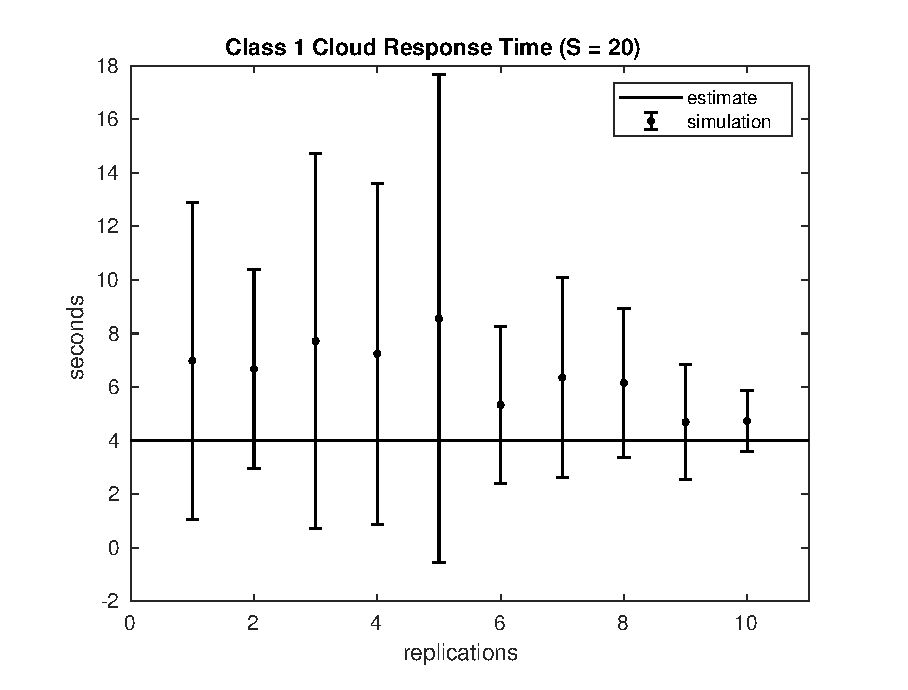
\includegraphics[width=\textwidth]{figures/simul/20_500K_s1cloud}
\caption{classe 1}
\label{20_s1cloud}
\end{subfigure}
%
\begin{subfigure}[t]{0.49\textwidth}
\includegraphics[width=\textwidth]{figures/simul/20_500K_s2cloud}
\caption{classe 2}
\label{20_s2cloud}
\end{subfigure}
%
\begin{subfigure}[t]{0.5\textwidth}
\includegraphics[width=\textwidth]{figures/simul/20_500K_scloud}
\caption{globale}
\label{20_scloud}
\end{subfigure}
%
\caption{tempo di risposta medio cloud per $S = 20$}
\end{figure}
%
\begin{table}[!h]
\begin{tabular}{c|r@{.}l|r@{.}l|r@{.}l}
& \multicolumn{2}{|c|}{$S_1^{cloud}$}
& \multicolumn{2}{|c|}{$S_2^{cloud}$}
& \multicolumn{2}{|c}{$S_{cloud}$} 
\\          
\hline
R1      & $6$&$9825 \pm 5.9108$   & $4$&$5450 \pm 0.0196$ & $4$&$5450 \pm 0.0195$ \\
R2      & $6$&$6797 \pm 3.7135$   & $4$&$5636 \pm 0.0219$ & $4$&$5633 \pm 0.0220$ \\
R3      & $7$&$7164 \pm 7.0027$   & $4$&$5644 \pm 0.0216$ & $4$&$5639 \pm 0.0211$ \\
R4      & $7$&$2403 \pm 6.3716$   & $4$&$5335 \pm 0.0185$ & $4$&$5329 \pm 0.0188$ \\
R5      & $8$&$5539 \pm 9.1042$   & $4$&$5436 \pm 0.0187$ & $4$&$5424 \pm 0.0185$ \\
R6      & $5$&$3354 \pm 2.9371$   & $4$&$5520 \pm 0.0221$ & $4$&$5510 \pm 0.0217$ \\
R7      & $6$&$3490 \pm 3.7333$   & $4$&$5626 \pm 0.0226$ & $4$&$5624 \pm 0.0226$ \\
R8      & $6$&$1600 \pm 2.7745$   & $4$&$5537 \pm 0.0195$ & $4$&$5532 \pm 0.0195$ \\
R9      & $4$&$6920 \pm 2.1527$   & $4$&$5409 \pm 0.0209$ & $4$&$5409 \pm 0.0204$ \\
R10     & $4$&$7340 \pm 1.1513$   & $4$&$5371 \pm 0.0197$ & $4$&$5374 \pm 0.0197$ \\
STIMA   & $4$&$0000$              & $4$&$5455$            & $4$&$5451$            \\
MAX ERR & $13$&$6581 \ (159.7\%)$ & $0$&$0406 \ (0.9\%)$  & $0$&$0402 \ (0.9\%)$    
\end{tabular}
\centering
\caption{Confronto tempi di risposta cloud per $S=20$}
\label{tab:20_scloud}
\end{table}

%%%%%%%%%%%%%%%%%%%%%%%%%%%%%%%%%%%%%%%%%%%%%%%%%%%%%%%%%%%%%%%%%%%%%%%%%%%%%%%%
\subsubsection{Tempi di risposta: Interruzioni}
%
\begin{figure}[!h]
\centering
%
\begin{subfigure}[t]{0.49\textwidth}
\includegraphics[width=\textwidth]{figures/simul/20_500K_intperc}
\caption{percentuale classe 2 interrotti}
\label{20_intperc}
\end{subfigure}
%
\begin{subfigure}[t]{0.49\textwidth}
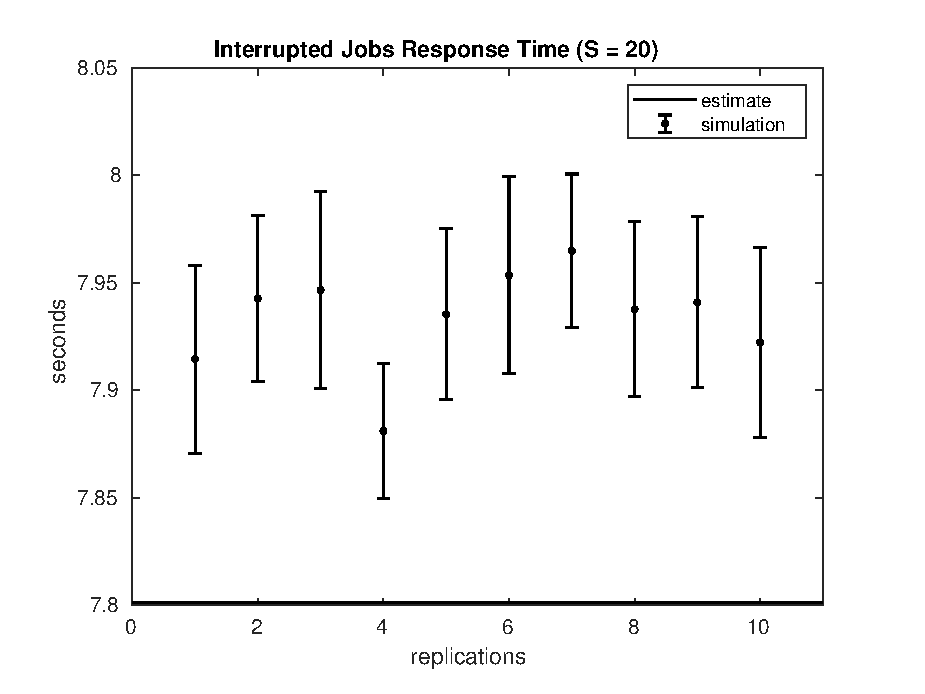
\includegraphics[width=\textwidth]{figures/simul/20_500K_sintr}
\caption{tempo di risposta job interrotti}
\label{20_s2cloud}
\end{subfigure}
%
\caption{statistice job interrotti per $S=20$}
\end{figure}
\begin{table}[!h]
\begin{tabular}{c|r@{.}l|r@{.}l}
& \multicolumn{2}{|c|}{\% interruzioni}
& \multicolumn{2}{|c}{$S_{intr}$}
\\          
\hline
R1      & $0$&$2394 \pm 0.0003$ & $7$&$9146 \pm 0.0437$ \\
R2      & $0$&$2395 \pm 0.0005$ & $7$&$9427 \pm 0.0387$ \\
R3      & $0$&$2381 \pm 0.0003$ & $7$&$9467 \pm 0.0458$ \\
R4      & $0$&$2371 \pm 0.0002$ & $7$&$8812 \pm 0.0312$ \\
R5      & $0$&$2416 \pm 0.0005$ & $7$&$9354 \pm 0.0398$ \\
R6      & $0$&$2388 \pm 0.0002$ & $7$&$9536 \pm 0.0457$ \\
R7      & $0$&$2392 \pm 0.0008$ & $7$&$9649 \pm 0.0358$ \\
R8      & $0$&$2381 \pm 0.0008$ & $7$&$9377 \pm 0.0407$ \\
R9      & $0$&$2376 \pm 0.0003$ & $7$&$9410 \pm 0.0397$ \\
R10     & $0$&$2385 \pm 0.0004$ & $7$&$9223 \pm 0.0443$ \\
STIMA   & $0$&$2280$            & $7$&$8016$            \\
MAX ERR & $0$&$0141 \ (5.8\%)$    & $0$&$1991 \ (2.5\%)$    
\end{tabular}
\centering
\caption{Confronto percentuale e tempi di risposta interruzioni per $S=20$}
\label{tab:20_sintr}
\end{table}

%%%%%%%%%%%%%%%%%%%%%%%%%%%%%%%%%%%%%%%%%%%%%%%%%%%%%%%%%%%%%%%%%%%%%%%%%%%%%%%%
\subsubsection{Tempi di risposta: Sistema}
%
\begin{figure}[!h]
\centering
%
\begin{subfigure}[t]{0.49\textwidth}
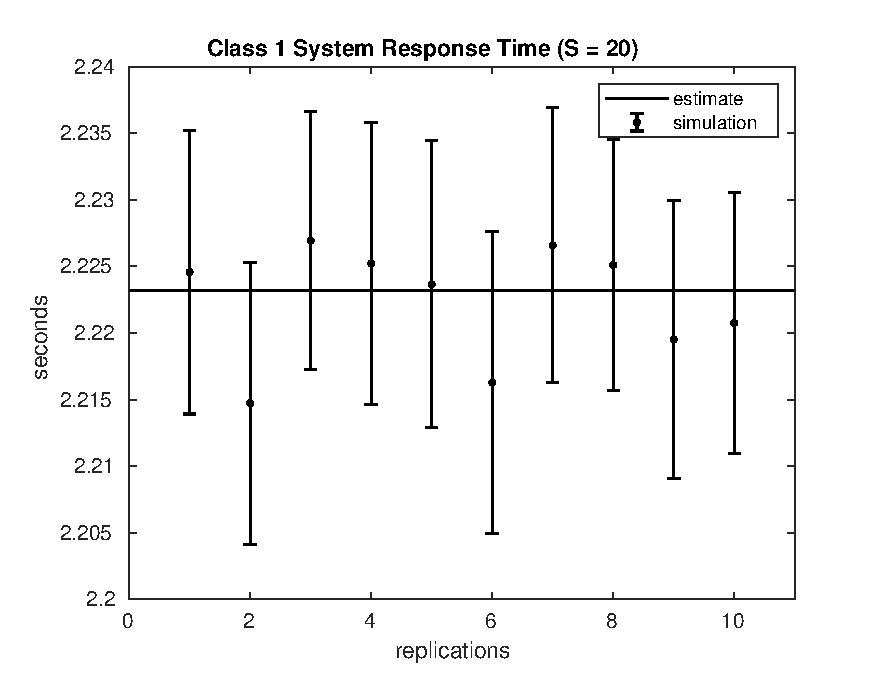
\includegraphics[width=\textwidth]{figures/simul/20_500K_s1}
\caption{classe 1}
\label{20_s1}
\end{subfigure}
%
\begin{subfigure}[t]{0.49\textwidth}
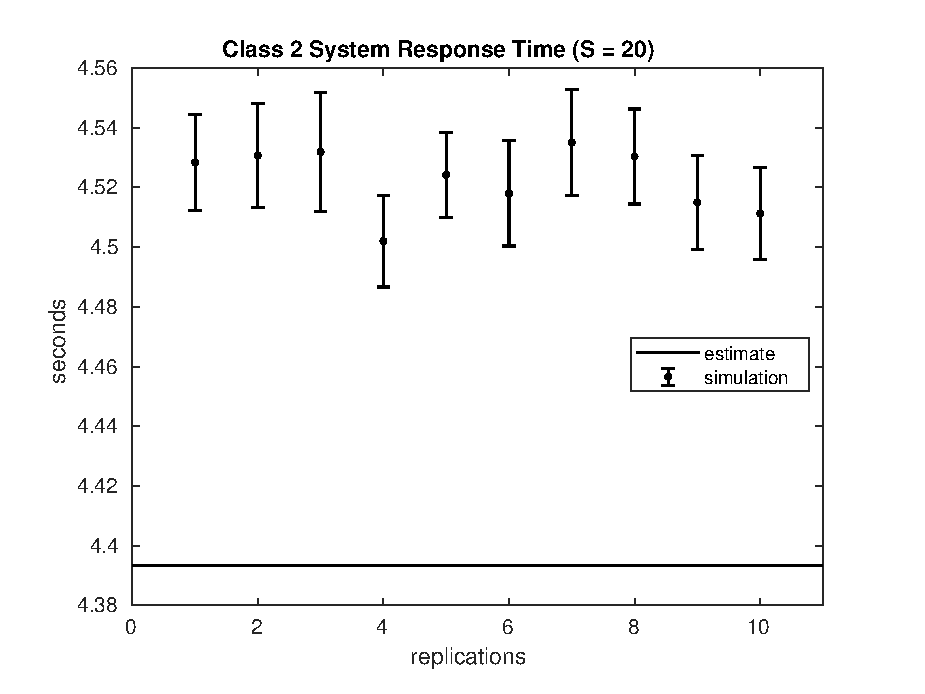
\includegraphics[width=\textwidth]{figures/simul/20_500K_s2}
\caption{classe 2}
\label{20_s2}
\end{subfigure}
%
\begin{subfigure}[t]{0.5\textwidth}
\includegraphics[width=\textwidth]{figures/simul/20_500K_s}
\caption{globale}
\label{20_s}
\end{subfigure}
%
\caption{tempo di risposta medio sistema per $S = 20$}
\end{figure}
%
\begin{table}[!h]
\begin{tabular}{c|r@{.}l|r@{.}l|r@{.}l}
& \multicolumn{2}{|c|}{$S_1$}
& \multicolumn{2}{|c|}{$S_2$}
& \multicolumn{2}{|c}{$S$} 
\\          
\hline
R1      & $2$&$2246 \pm 0.0107$ & $4$&$5284 \pm 0.0160$ & $3$&$6266 \pm 0.0096$ \\
R2      & $2$&$2147 \pm 0.0106$ & $4$&$5307 \pm 0.0174$ & $3$&$6269 \pm 0.0121$ \\
R3      & $2$&$2269 \pm 0.0097$ & $4$&$5319 \pm 0.0199$ & $3$&$6307 \pm 0.0133$ \\
R4      & $2$&$2252 \pm 0.0106$ & $4$&$5020 \pm 0.0154$ & $3$&$6124 \pm 0.0110$ \\
R5      & $2$&$2237 \pm 0.0108$ & $4$&$5242 \pm 0.0142$ & $3$&$6218 \pm 0.0097$ \\
R6      & $2$&$2163 \pm 0.0113$ & $4$&$5180 \pm 0.0176$ & $3$&$6197 \pm 0.0125$ \\
R7      & $2$&$2266 \pm 0.0103$ & $4$&$5351 \pm 0.0177$ & $3$&$6344 \pm 0.0119$ \\
R8      & $2$&$2251 \pm 0.0094$ & $4$&$5303 \pm 0.0159$ & $3$&$6318 \pm 0.0103$ \\
R9      & $2$&$2195 \pm 0.0104$ & $4$&$5150 \pm 0.0157$ & $3$&$6193 \pm 0.0109$ \\
R10     & $2$&$2208 \pm 0.0098$ & $4$&$5113 \pm 0.0155$ & $3$&$6152 \pm 0.0100$ \\
STIMA   & $2$&$2232$            & $4$&$3935$            & $3$&$5465$            \\
MAX ERR & $0$&$0137 \ (0.6\%)$    & $0$&$1593 \ (3.5\%)$    & $0$&$0999 \ (2.7\%)$    
\end{tabular}
\centering
\caption{Confronto tempi di risposta sistema per $S=20$}
\label{tab:20_s}
\end{table}

%%%%%%%%%%%%%%%%%%%%%%%%%%%%%%%%%%%%%%%%%%%%%%%%%%%%%%%%%%%%%%%%%%%%%%%%%%%%%%%%
\subsubsection{Popolazione: Cloudlet}
%
\begin{figure}[!h]
\centering
%
\begin{subfigure}[t]{0.49\textwidth}
\includegraphics[width=\textwidth]{figures/simul/20_500K_n1clet}
\caption{classe 1}
\label{20_n1clet}
\end{subfigure}
%
\begin{subfigure}[t]{0.49\textwidth}
\includegraphics[width=\textwidth]{figures/simul/20_500K_n2clet}
\caption{classe 2}
\label{20_n2clet}
\end{subfigure}
%
\begin{subfigure}[t]{0.5\textwidth}
\includegraphics[width=\textwidth]{figures/simul/20_500K_nclet}
\caption{globale}
\label{20_nclet}
\end{subfigure}
%
\caption{popolazione media cloudlet per $S = 20$}
\end{figure}
%
\begin{table}[!h]
\begin{tabular}{c|r@{.}l|r@{.}l|r@{.}l}
& \multicolumn{2}{|c|}{$N_1^{clet}$}
& \multicolumn{2}{|c|}{$N_2^{clet}$}
& \multicolumn{2}{|c}{$N_{clet}$} 
\\          
\hline
R1      & $8$&$9175 \pm 0.0070$ & $9$&$6707 \pm 0.0069$ & $18$&$5882 \pm 0.0035$ \\
R2      & $8$&$8757 \pm 0.0154$ & $9$&$6856 \pm 0.0183$ & $18$&$5614 \pm 0.0112$ \\
R3      & $8$&$9431 \pm 0.0074$ & $9$&$6394 \pm 0.0059$ & $18$&$5825 \pm 0.0059$ \\
R4      & $8$&$8371 \pm 0.0222$ & $9$&$7394 \pm 0.0208$ & $18$&$5765 \pm 0.0035$ \\
R5      & $8$&$9625 \pm 0.0149$ & $9$&$6128 \pm 0.0188$ & $18$&$5753 \pm 0.0047$ \\
R6      & $8$&$8553 \pm 0.0072$ & $9$&$7140 \pm 0.0089$ & $18$&$5693 \pm 0.0041$ \\
R7      & $8$&$9466 \pm 0.0131$ & $9$&$6312 \pm 0.0120$ & $18$&$5779 \pm 0.0033$ \\
R8      & $8$&$8924 \pm 0.0302$ & $9$&$6854 \pm 0.0230$ & $18$&$5778 \pm 0.0084$ \\
R9      & $8$&$8399 \pm 0.0127$ & $9$&$7243 \pm 0.0092$ & $18$&$5642 \pm 0.0057$ \\
R10     & $8$&$8683 \pm 0.0112$ & $9$&$7099 \pm 0.0093$ & $18$&$5782 \pm 0.0026$ \\
STIMA   & $8$&$8841$            & $9$&$6087$            & $18$&$4928$            \\
MAX ERR & $0$&$0933 \ (1.0\%)$  & $0$&$1515 \ (1.6\%)$  & $0$&$0988 \ (0.5\%)$     
\end{tabular}
\centering
\caption{Confronto popolazione cloudlet per $S=20$}
\label{tab:20_nclet}
\end{table}

%%%%%%%%%%%%%%%%%%%%%%%%%%%%%%%%%%%%%%%%%%%%%%%%%%%%%%%%%%%%%%%%%%%%%%%%%%%%%%%%
\subsubsection{Popolazione: Cloud}
%
\begin{figure}[!h]
\centering
%
\begin{subfigure}[t]{0.49\textwidth}
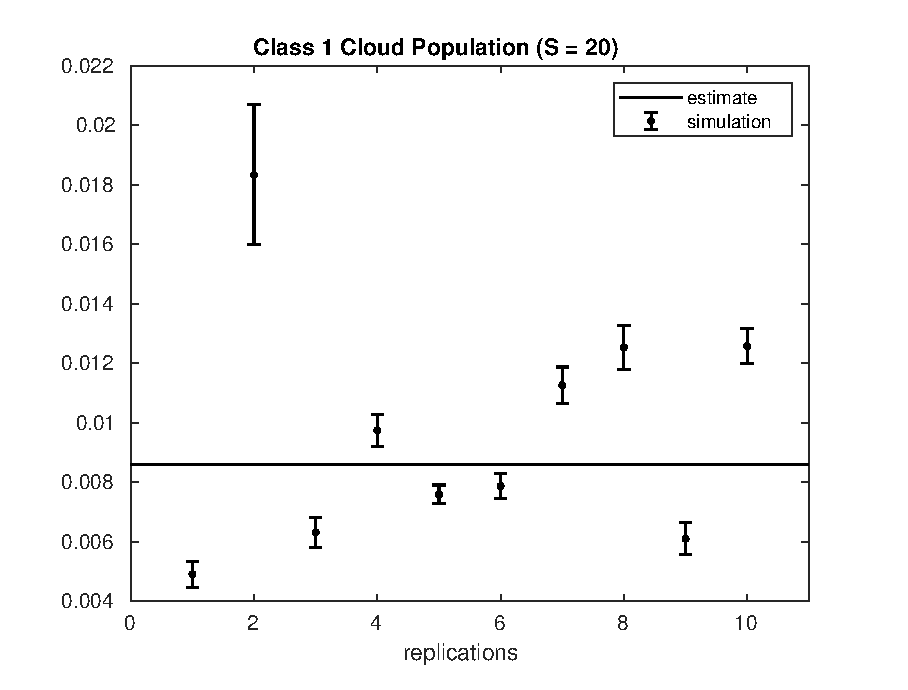
\includegraphics[width=\textwidth]{figures/simul/20_500K_n1cloud}
\caption{classe 1}
\label{20_n1cloud}
\end{subfigure}
%
\begin{subfigure}[t]{0.49\textwidth}
\includegraphics[width=\textwidth]{figures/simul/20_500K_n2cloud}
\caption{classe 2}
\label{20_n2cloud}
\end{subfigure}
%
\begin{subfigure}[t]{0.5\textwidth}
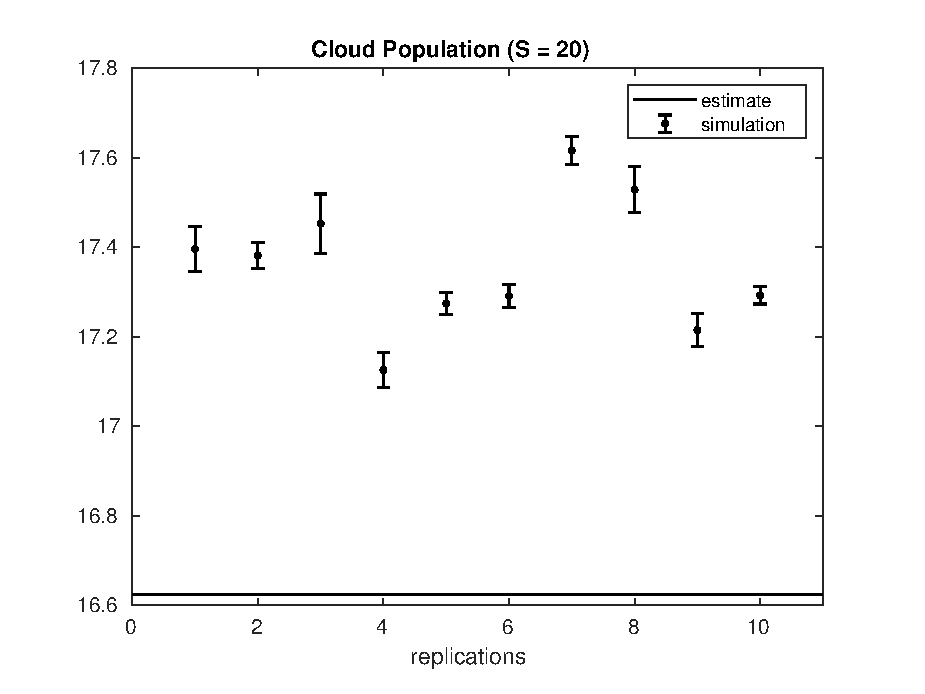
\includegraphics[width=\textwidth]{figures/simul/20_500K_ncloud}
\caption{globale}
\label{20_ncloud}
\end{subfigure}
%
\caption{popolazione media cloud per $S = 20$}
\end{figure}
%
\begin{table}[!h]
\begin{tabular}{c|r@{.}l|r@{.}l|r@{.}l}
& \multicolumn{2}{|c|}{$N_1^{cloud}$}
& \multicolumn{2}{|c|}{$N_2^{cloud}$}
& \multicolumn{2}{|c}{$N_{cloud}$} 
\\          
\hline
R1      & $0$&$0049 \pm 0.0004$ & $17$&$3911 \pm 0.0508$ & $17$&$3960 \pm 0.0510$ \\
R2      & $0$&$0183 \pm 0.0024$ & $17$&$3631 \pm 0.0287$ & $17$&$3814 \pm 0.0288$ \\
R3      & $0$&$0063 \pm 0.0005$ & $17$&$4461 \pm 0.0659$ & $17$&$4524 \pm 0.0662$ \\
R4      & $0$&$0097 \pm 0.0005$ & $17$&$1158 \pm 0.0384$ & $17$&$1256 \pm 0.0387$ \\
R5      & $0$&$0076 \pm 0.0003$ & $17$&$2666 \pm 0.0249$ & $17$&$2742 \pm 0.0247$ \\
R6      & $0$&$0079 \pm 0.0004$ & $17$&$2828 \pm 0.0251$ & $17$&$2907 \pm 0.0253$ \\
R7      & $0$&$0113 \pm 0.0006$ & $17$&$6046 \pm 0.0309$ & $17$&$6158 \pm 0.0314$ \\
R8      & $0$&$0125 \pm 0.0007$ & $17$&$5160 \pm 0.0511$ & $17$&$5285 \pm 0.0515$ \\
R9      & $0$&$0061 \pm 0.0005$ & $17$&$2087 \pm 0.0371$ & $17$&$2148 \pm 0.0368$ \\
R10     & $0$&$0126 \pm 0.0006$ & $17$&$2797 \pm 0.0190$ & $17$&$2923 \pm 0.0192$ \\
STIMA   & $0$&$0086$            & $16$&$6166$            & $16$&$6252$            \\
MAX ERR & $0$&$0121 \ (65.9\%)$ & $1$&$0188 \ (5.8\%)$   & $1$&$0220 \ (5.8\%)$     
\end{tabular}
\centering
\caption{Confronto popolazione cloud per $S=20$}
\label{tab:20_ncloud}
\end{table}

%%%%%%%%%%%%%%%%%%%%%%%%%%%%%%%%%%%%%%%%%%%%%%%%%%%%%%%%%%%%%%%%%%%%%%%%%%%%%%%%
\subsubsection{Popolazione: Sistema}
%
\begin{figure}[!h]
\centering
%
\begin{subfigure}[t]{0.49\textwidth}
\includegraphics[width=\textwidth]{figures/simul/20_500K_n1}
\caption{classe 1}
\label{20_n1}
\end{subfigure}
%
\begin{subfigure}[t]{0.49\textwidth}
\includegraphics[width=\textwidth]{figures/simul/20_500K_n2}
\caption{classe 2}
\label{20_n2}
\end{subfigure}
%
\begin{subfigure}[t]{0.5\textwidth}
\includegraphics[width=\textwidth]{figures/simul/20_500K_n}
\caption{globale}
\label{20_n}
\end{subfigure}
%
\caption{popolazione media sistema per $S = 20$}
\end{figure}
%
\begin{table}[!h]
\begin{tabular}{c|r@{.}l|r@{.}l|r@{.}l}
& \multicolumn{2}{|c|}{$N_1$}
& \multicolumn{2}{|c|}{$N_2$}
& \multicolumn{2}{|c}{$N$} 
\\          
\hline
R1      & $8$&$9224 \pm 0.0071$ & $28$&$2635 \pm 0.0541$ & $37$&$1859 \pm 0.0541$ \\
R2      & $8$&$8941 \pm 0.0171$ & $28$&$2474 \pm 0.0404$ & $37$&$1415 \pm 0.0420$ \\
R3      & $8$&$9494 \pm 0.0077$ & $28$&$2872 \pm 0.0677$ & $37$&$2366 \pm 0.0733$ \\
R4      & $8$&$8469 \pm 0.0225$ & $28$&$0382 \pm 0.0221$ & $36$&$8850 \pm 0.0400$ \\
R5      & $8$&$9701 \pm 0.0150$ & $28$&$0775 \pm 0.0377$ & $37$&$0476 \pm 0.0271$ \\
R6      & $8$&$8632 \pm 0.0072$ & $28$&$1899 \pm 0.0292$ & $37$&$0531 \pm 0.0303$ \\
R7      & $8$&$9579 \pm 0.0131$ & $28$&$4456 \pm 0.0258$ & $37$&$4034 \pm 0.0309$ \\
R8      & $8$&$9049 \pm 0.0307$ & $28$&$3933 \pm 0.0390$ & $37$&$2982 \pm 0.0629$ \\
R9      & $8$&$8460 \pm 0.0130$ & $28$&$1278 \pm 0.0378$ & $36$&$9738 \pm 0.0406$ \\
R10     & $8$&$8808 \pm 0.0117$ & $28$&$1810 \pm 0.0169$ & $37$&$0619 \pm 0.0203$ \\
STIMA   & $8$&$8927$            & $27$&$4591$            & $36$&$3518$            \\
MAX ERR & $0$&$0925 \ (1.0\%)$  & $1$&$0122 \ (3.6\%)$   & $1$&$0825 \ (2.9\%)$     
\end{tabular}
\centering
\caption{Confronto popolazione sistema per $S=20$}
\label{tab:20_n}
\end{table}

%%%%%%%%%%%%%%%%%%%%%%%%%%%%%%%%%%%%%%%%%%%%%%%%%%%%%%%%%%%%%%%%%%%%%%%%%%%%%%%%
\subsubsection{Throughput: Cloudlet}
%
\begin{figure}[!h]
\centering
%
\begin{subfigure}[t]{0.49\textwidth}
\includegraphics[width=\textwidth]{figures/simul/20_500K_x1clet}
\caption{classe 1}
\label{20_x1clet}
\end{subfigure}
%
\begin{subfigure}[t]{0.49\textwidth}
\includegraphics[width=\textwidth]{figures/simul/20_500K_x2clet}
\caption{classe 2}
\label{20_x2clet}
\end{subfigure}
%
\begin{subfigure}[t]{0.5\textwidth}
\includegraphics[width=\textwidth]{figures/simul/20_500K_xclet}
\caption{globale}
\label{20_xclet}
\end{subfigure}
%
\caption{throughput cloudlet per $S = 20$}
\end{figure}
%
\begin{table}[!h]
\begin{tabular}{c|r@{.}l|r@{.}l|r@{.}l}
& \multicolumn{2}{|c|}{$X_1^{clet}$}
& \multicolumn{2}{|c|}{$X_2^{clet}$}
& \multicolumn{2}{|c}{$X_{clet}$} 
\\          
\hline
R1      & $4$&$0054 \pm 0.0043$ & $2$&$4201 \pm 0.0027$ & $6$&$4255 \pm 0.0042$ \\
R2      & $4$&$0021 \pm 0.0048$ & $2$&$4234 \pm 0.0058$ & $6$&$4255 \pm 0.0030$ \\
R3      & $4$&$0171 \pm 0.0020$ & $2$&$4338 \pm 0.0064$ & $6$&$4510 \pm 0.0057$ \\
R4      & $3$&$9768 \pm 0.0043$ & $2$&$4438 \pm 0.0019$ & $6$&$4207 \pm 0.0036$ \\
R5      & $4$&$0247 \pm 0.0027$ & $2$&$3972 \pm 0.0066$ & $6$&$4219 \pm 0.0057$ \\
R6      & $4$&$0015 \pm 0.0022$ & $2$&$4397 \pm 0.0048$ & $6$&$4412 \pm 0.0043$ \\
R7      & $4$&$0223 \pm 0.0072$ & $2$&$4164 \pm 0.0044$ & $6$&$4387 \pm 0.0041$ \\
R8      & $3$&$9935 \pm 0.0108$ & $2$&$4257 \pm 0.0084$ & $6$&$4193 \pm 0.0033$ \\
R9      & $3$&$9824 \pm 0.0032$ & $2$&$4452 \pm 0.0044$ & $6$&$4276 \pm 0.0050$ \\
R10     & $4$&$0005 \pm 0.0033$ & $2$&$4267 \pm 0.0035$ & $6$&$4272 \pm 0.0021$ \\
STIMA   & $3$&$9978$            & $2$&$5943$            & $6$&$5922$            \\
MAX ERR & $0$&$0317 \ (0.8\%)$  & $0$&$1905 \ (7.9\%)$  & $0$&$1696 \ (2.6\%)$    
\end{tabular}
\centering
\caption{Confronto throughput cloudlet per $S=20$}
\label{tab:20_xclet}
\end{table}

%%%%%%%%%%%%%%%%%%%%%%%%%%%%%%%%%%%%%%%%%%%%%%%%%%%%%%%%%%%%%%%%%%%%%%%%%%%%%%%%
\subsubsection{Throughput: Cloud}
%
\begin{figure}[!h]
\centering
%
\begin{subfigure}[t]{0.49\textwidth}
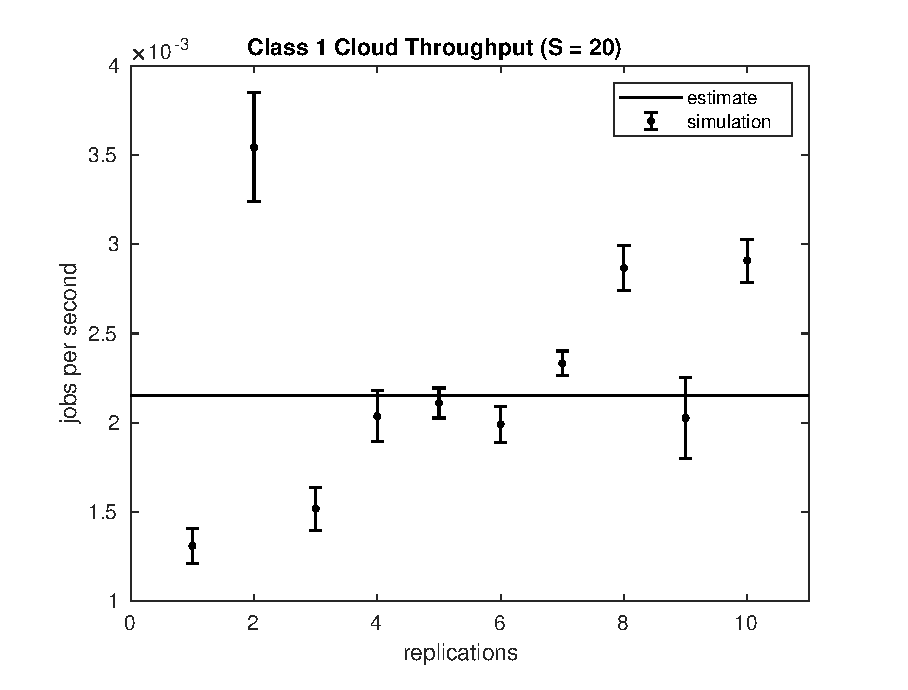
\includegraphics[width=\textwidth]{figures/simul/20_500K_x1cloud}
\caption{classe 1}
\label{20_x1cloud}
\end{subfigure}
%
\begin{subfigure}[t]{0.49\textwidth}
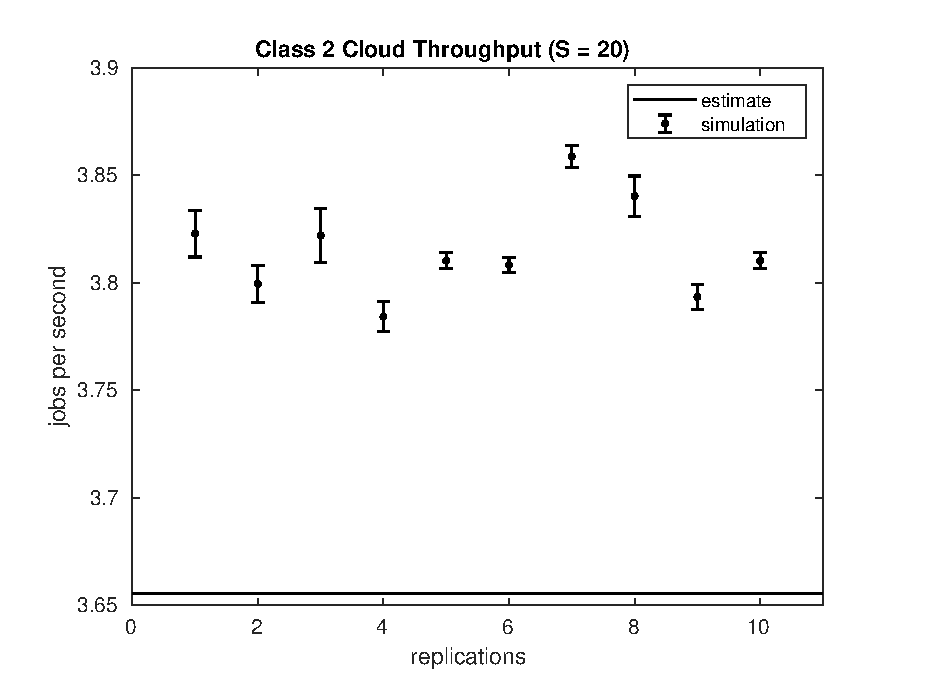
\includegraphics[width=\textwidth]{figures/simul/20_500K_x2cloud}
\caption{classe 2}
\label{20_x2cloud}
\end{subfigure}
%
\begin{subfigure}[t]{0.5\textwidth}
\includegraphics[width=\textwidth]{figures/simul/20_500K_xcloud}
\caption{globale}
\label{20_xcloud}
\end{subfigure}
%
\caption{throughput cloud per $S = 20$}
\end{figure}
%
\begin{table}[!h]
\begin{tabular}{c|r@{.}l|r@{.}l|r@{.}l}
& \multicolumn{2}{|c|}{$X_1^{cloud}$}
& \multicolumn{2}{|c|}{$X_2^{cloud}$}
& \multicolumn{2}{|c}{$X_{cloud}$} 
\\          
\hline
R1      & $0$&$0013 \pm 0.0001$ & $3$&$8230 \pm 0.0109$ & $3$&$8243 \pm 0.0109$ \\
R2      & $0$&$0035 \pm 0.0003$ & $3$&$7996 \pm 0.0086$ & $3$&$8031 \pm 0.0085$ \\
R3      & $0$&$0015 \pm 0.0001$ & $3$&$8221 \pm 0.0127$ & $3$&$8236 \pm 0.0128$ \\
R4      & $0$&$0020 \pm 0.0001$ & $3$&$7843 \pm 0.0069$ & $3$&$7864 \pm 0.0070$ \\
R5      & $0$&$0021 \pm 0.0001$ & $3$&$8103 \pm 0.0036$ & $3$&$8124 \pm 0.0037$ \\
R6      & $0$&$0020 \pm 0.0001$ & $3$&$8084 \pm 0.0036$ & $3$&$8104 \pm 0.0036$ \\
R7      & $0$&$0023 \pm 0.0001$ & $3$&$8588 \pm 0.0050$ & $3$&$8612 \pm 0.0051$ \\
R8      & $0$&$0029 \pm 0.0001$ & $3$&$8404 \pm 0.0093$ & $3$&$8433 \pm 0.0094$ \\
R9      & $0$&$0020 \pm 0.0002$ & $3$&$7935 \pm 0.0058$ & $3$&$7955 \pm 0.0057$ \\
R10     & $0$&$0029 \pm 0.0001$ & $3$&$8103 \pm 0.0037$ & $3$&$8132 \pm 0.0037$ \\
STIMA   & $0$&$0022$            & $3$&$6557$            & $3$&$6578$            \\
MAX ERR & $0$&$0017 \ (47.9\%)$ & $0$&$2082 \ (5.4\%)$  & $0$&$2084 \ (5.4\%)$    
\end{tabular}
\centering
\caption{Confronto throughput cloud per $S=20$}
\label{tab:20_xcloud}
\end{table}

%%%%%%%%%%%%%%%%%%%%%%%%%%%%%%%%%%%%%%%%%%%%%%%%%%%%%%%%%%%%%%%%%%%%%%%%%%%%%%%%
\subsubsection{Throughput: Sistema}
%
\begin{figure}[!h]
\centering
%
\begin{subfigure}[t]{0.49\textwidth}
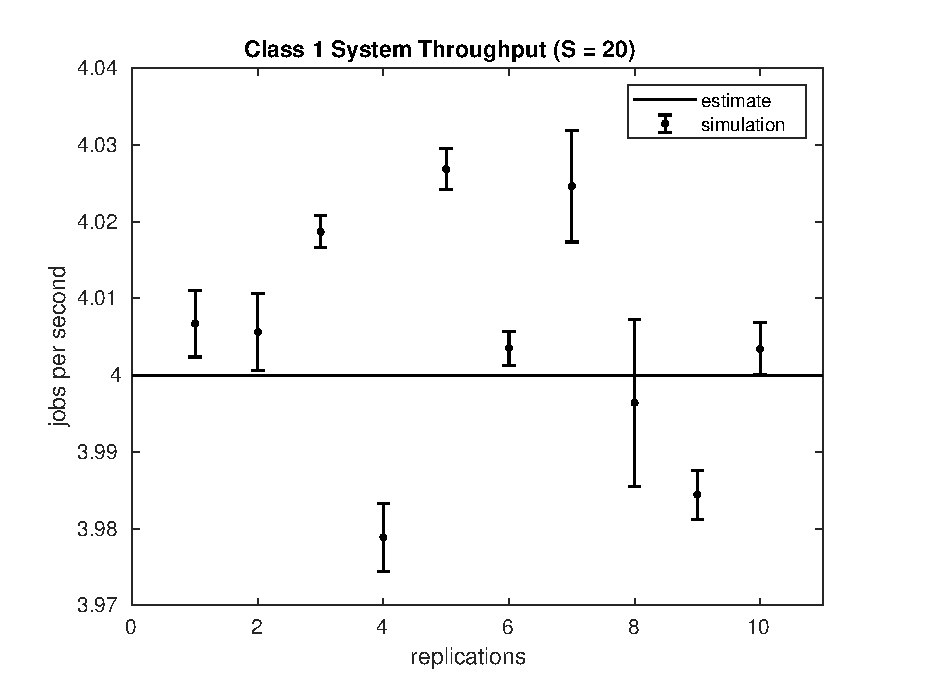
\includegraphics[width=\textwidth]{figures/simul/20_500K_x1}
\caption{classe 1}
\label{20_x1}
\end{subfigure}
%
\begin{subfigure}[t]{0.49\textwidth}
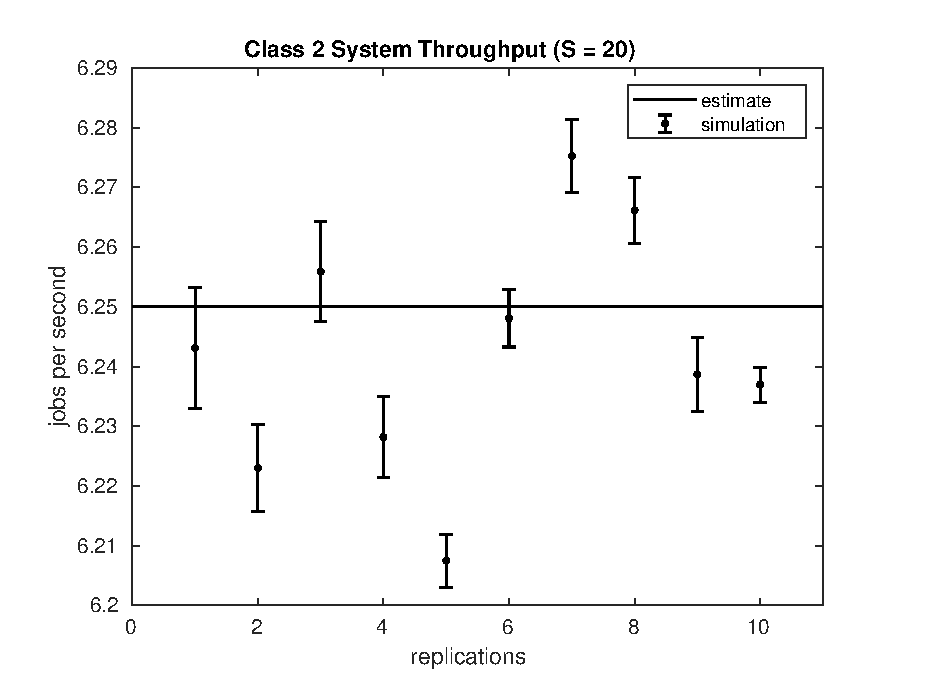
\includegraphics[width=\textwidth]{figures/simul/20_500K_x2}
\caption{classe 2}
\label{20_x2}
\end{subfigure}
%
\begin{subfigure}[t]{0.5\textwidth}
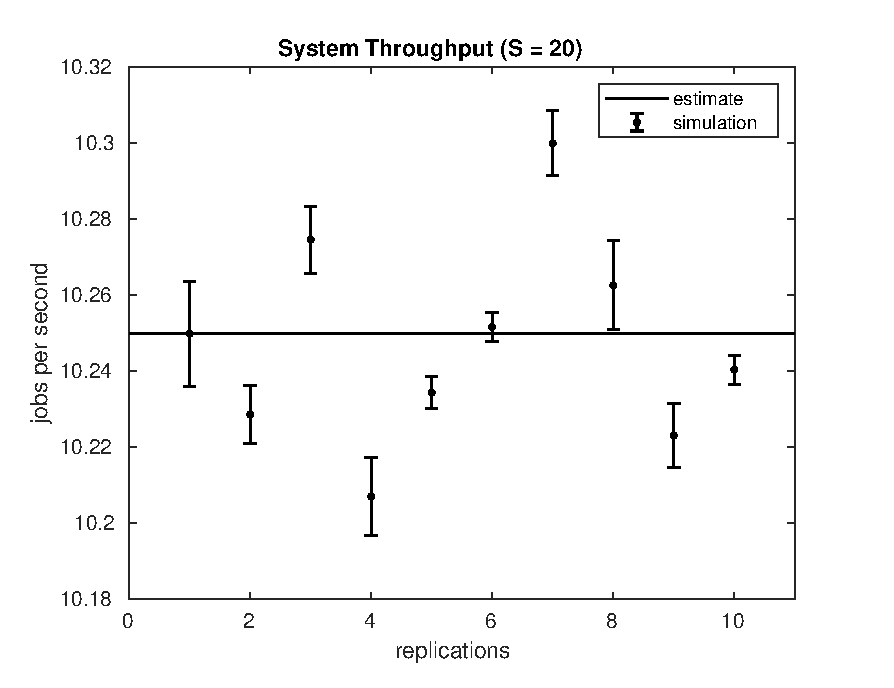
\includegraphics[width=\textwidth]{figures/simul/20_500K_x}
\caption{globale}
\label{20_x}
\end{subfigure}
%
\caption{throughput sistema per $S = 20$}
\end{figure}
%
\begin{table}[!h]
\begin{tabular}{c|r@{.}l|r@{.}l|r@{.}l}
& \multicolumn{2}{|c|}{$X_1$}
& \multicolumn{2}{|c|}{$X_2$}
& \multicolumn{2}{|c}{$X$} 
\\          
\hline
R1      & $4$&$0067 \pm 0.0044$ & $6$&$2431 \pm 0.0101$ & $10$&$2498 \pm 0.0138$ \\
R2      & $4$&$0056 \pm 0.0050$ & $6$&$2230 \pm 0.0072$ & $10$&$2286 \pm 0.0076$ \\
R3      & $4$&$0187 \pm 0.0021$ & $6$&$2559 \pm 0.0083$ & $10$&$2746 \pm 0.0088$ \\
R4      & $3$&$9789 \pm 0.0044$ & $6$&$2282 \pm 0.0068$ & $10$&$2071 \pm 0.0102$ \\
R5      & $4$&$0268 \pm 0.0027$ & $6$&$2075 \pm 0.0044$ & $10$&$2343 \pm 0.0042$ \\
R6      & $4$&$0035 \pm 0.0022$ & $6$&$2481 \pm 0.0048$ & $10$&$2516 \pm 0.0039$ \\
R7      & $4$&$0246 \pm 0.0073$ & $6$&$2753 \pm 0.0061$ & $10$&$2999 \pm 0.0086$ \\
R8      & $3$&$9964 \pm 0.0109$ & $6$&$2661 \pm 0.0055$ & $10$&$2625 \pm 0.0117$ \\
R9      & $3$&$9844 \pm 0.0032$ & $6$&$2387 \pm 0.0061$ & $10$&$2231 \pm 0.0085$ \\
R10     & $4$&$0034 \pm 0.0034$ & $6$&$2370 \pm 0.0029$ & $10$&$2404 \pm 0.0038$ \\
STIMA   & $4$&$0000$            & $6$&$2500$            & $10$&$2500$            \\
MAX ERR & $0$&$0319 \ (0.8\%)$  & $0$&$0381 \ (0.6\%)$  & $0$&$0584 \ (0.6\%)$     
\end{tabular}
\centering
\caption{Confronto throughput sistema per $S=20$}
\label{tab:20_x}
\end{table}

%
%
%%%%%%%%%%%%%%%%%%%%%%%%%%%%%%%%%%%%%%%%%%%%%%%%%%%%%%%%%%%%%%%%%%%%%%%%%%%%%%%%
%%%%%%%%%%%%%%%%%%%%%%%%%%%%%%%%%%%%%%%%%%%%%%%%%%%%%%%%%%%%%%%%%%%%%%%%%%%%%%%%
\subsection{Scenario 2: $\mathbf{S=\frac{N}{2}=10}$}
\subsubsection{Tempi di risposta: Cloudlet}
%
\begin{figure}[!h]
\centering
%
\begin{subfigure}[t]{0.49\textwidth}
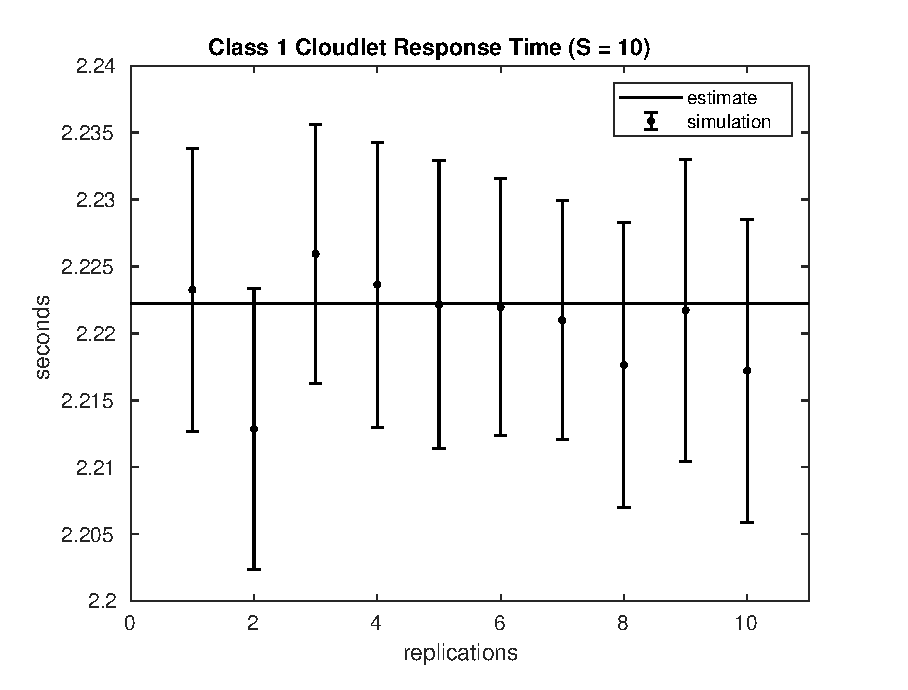
\includegraphics[width=\textwidth]{figures/simul/10_500K_s1clet}
\caption{classe 1}
\label{10_s1clet}
\end{subfigure}
%
\begin{subfigure}[t]{0.49\textwidth}
\includegraphics[width=\textwidth]{figures/simul/10_500K_s2clet}
\caption{classe 2}
\label{10_s2clet}
\end{subfigure}
%
\begin{subfigure}[t]{0.5\textwidth}
\includegraphics[width=\textwidth]{figures/simul/10_500K_sclet}
\caption{globale}
\label{10_sclet}
\end{subfigure}
%
\caption{tempo di risposta medio cloudlet per $S = 10$}
\end{figure}
%
\begin{table}[!h]
\begin{tabular}{c|r@{.}l|r@{.}l|r@{.}l}
& \multicolumn{2}{|c|}{$S_1^{clet}$}
& \multicolumn{2}{|c|}{$S_2^{clet}$}
& \multicolumn{2}{|c}{$S_{clet}$} 
\\          
\hline
R1      & $2$&$2233 \pm 0.0106$ & $0$&$8151 \pm 0.0187$ & $2$&$1240 \pm 0.0115$ \\
R2      & $2$&$2129 \pm 0.0105$ & $0$&$8441 \pm 0.0228$ & $2$&$1123 \pm 0.0115$ \\
R3      & $2$&$2259 \pm 0.0097$ & $0$&$7968 \pm 0.0199$ & $2$&$1265 \pm 0.0104$ \\
R4      & $2$&$2236 \pm 0.0106$ & $0$&$8314 \pm 0.0185$ & $2$&$1213 \pm 0.0114$ \\
R5      & $2$&$2222 \pm 0.0107$ & $0$&$8237 \pm 0.0203$ & $2$&$1221 \pm 0.0110$ \\
R6      & $2$&$2220 \pm 0.0096$ & $0$&$8139 \pm 0.0196$ & $2$&$1204 \pm 0.0102$ \\
R7      & $2$&$2210 \pm 0.0089$ & $0$&$8136 \pm 0.0173$ & $2$&$1216 \pm 0.0103$ \\
R8      & $2$&$2177 \pm 0.0107$ & $0$&$8197 \pm 0.0186$ & $2$&$1151 \pm 0.0112$ \\
R9      & $2$&$2217 \pm 0.0113$ & $0$&$8232 \pm 0.0241$ & $2$&$1191 \pm 0.0115$ \\
R10     & $2$&$2172 \pm 0.0113$ & $0$&$8296 \pm 0.0242$ & $2$&$1141 \pm 0.0127$ \\
STIMA   & $2$&$2222$            & $0$&$8425$            & $2$&$1002$            \\
MAX ERR & $0$&$0134 \ (0.6\%)$  & $0$&$0258 \ (3.2\%)$  & $0$&$0367 \ (1.7\%)$    
\end{tabular}
\centering
\caption{Confronto tempi risposta cloudlet per $S=10$}
\label{tab:10_sclet}
\end{table}

%%%%%%%%%%%%%%%%%%%%%%%%%%%%%%%%%%%%%%%%%%%%%%%%%%%%%%%%%%%%%%%%%%%%%%%%%%%%%%%%
\subsubsection{Tempi di risposta: Cloud}
%
\begin{figure}[!h]
\centering
%
\begin{subfigure}[t]{0.49\textwidth}
\includegraphics[width=\textwidth]{figures/simul/10_500K_s1cloud}
\caption{classe 1}
\label{10_s1cloud}
\end{subfigure}
%
\begin{subfigure}[t]{0.49\textwidth}
\includegraphics[width=\textwidth]{figures/simul/10_500K_s2cloud}
\caption{classe 2}
\label{10_s2cloud}
\end{subfigure}
%
\begin{subfigure}[t]{0.5\textwidth}
\includegraphics[width=\textwidth]{figures/simul/10_500K_scloud}
\caption{globale}
\label{10_scloud}
\end{subfigure}
%
\caption{tempo di risposta medio cloud per $S = 10$}
\end{figure}
%
\begin{table}[!h]
\begin{tabular}{c|r@{.}l|r@{.}l|r@{.}l}
& \multicolumn{2}{|c|}{$S_1^{cloud}$}
& \multicolumn{2}{|c|}{$S_2^{cloud}$}
& \multicolumn{2}{|c}{$S_{cloud}$} 
\\          
\hline
R1      & $5$&$5360 \pm 3.1331$   & $4$&$5460 \pm 0.0188$ & $4$&$5455 \pm 0.0187$ \\
R2      & $7$&$4166 \pm 4.7422$   & $4$&$5591 \pm 0.0179$ & $4$&$5583 \pm 0.0181$ \\
R3      & $3$&$9017 \pm 0.9934$   & $4$&$5597 \pm 0.0165$ & $4$&$5591 \pm 0.0164$ \\
R4      & $6$&$5053 \pm 3.8063$   & $4$&$5376 \pm 0.0154$ & $4$&$5370 \pm 0.0157$ \\
R5      & $6$&$3977 \pm 4.5474$   & $4$&$5560 \pm 0.0148$ & $4$&$5553 \pm 0.0146$ \\
R6      & $4$&$2407 \pm 1.0694$   & $4$&$5512 \pm 0.0183$ & $4$&$5506 \pm 0.0183$ \\
R7      & $4$&$3667 \pm 0.7650$   & $4$&$5353 \pm 0.0186$ & $4$&$5351 \pm 0.0186$ \\
R8      & $7$&$8029 \pm 7.5835$   & $4$&$5308 \pm 0.0156$ & $4$&$5301 \pm 0.0158$ \\
R9      & $7$&$2376 \pm 5.1424$   & $4$&$5480 \pm 0.0157$ & $4$&$5478 \pm 0.0159$ \\
R10     & $6$&$9964 \pm 6.2793$   & $4$&$5319 \pm 0.0151$ & $4$&$5315 \pm 0.0151$ \\
STIMA   & $4$&$0000$              & $4$&$5455$            & $4$&$5453$            \\
MAX ERR & $11$&$3864 \ (145.9\%)$ & $0$&$0316 \ (0.7\%)$  & $0$&$0312 \ (0.7\%)$    
\end{tabular}
\centering
\caption{Confronto tempi di risposta cloud per $S=10$}
\label{tab:10_scloud}
\end{table}

%%%%%%%%%%%%%%%%%%%%%%%%%%%%%%%%%%%%%%%%%%%%%%%%%%%%%%%%%%%%%%%%%%%%%%%%%%%%%%%%
\subsubsection{Tempi di risposta: Interruzioni}
%
\begin{figure}[!h]
\centering
%
\begin{subfigure}[t]{0.49\textwidth}
\includegraphics[width=\textwidth]{figures/simul/10_500K_intperc}
\caption{percentuale classe 2 interrotti}
\label{10_intperc}
\end{subfigure}
%
\begin{subfigure}[t]{0.49\textwidth}
\includegraphics[width=\textwidth]{figures/simul/10_500K_sintr}
\caption{tempo di risposta job interrotti}
\label{10_s2cloud}
\end{subfigure}
%
\caption{statistice job interrotti per $S=10$}
\end{figure}
\begin{table}[!h]
\begin{tabular}{c|r@{.}l|r@{.}l}
& \multicolumn{2}{|c|}{\% interruzioni}
& \multicolumn{2}{|c}{$S_{intr}$}
\\          
\hline
R1      & $0$&$2153 \pm 0.0004$ & $6$&$2006 \pm 0.0381$ \\
R2      & $0$&$2148 \pm 0.0005$ & $6$&$2496 \pm 0.0401$ \\
R3      & $0$&$2140 \pm 0.0007$ & $6$&$2580 \pm 0.0342$ \\
R4      & $0$&$2186 \pm 0.0013$ & $6$&$2358 \pm 0.0377$ \\
R5      & $0$&$2129 \pm 0.0005$ & $6$&$2184 \pm 0.0373$ \\
R6      & $0$&$2170 \pm 0.0008$ & $6$&$2206 \pm 0.0383$ \\
R7      & $0$&$2130 \pm 0.0009$ & $6$&$2275 \pm 0.0441$ \\
R8      & $0$&$2177 \pm 0.0005$ & $6$&$1910 \pm 0.0386$ \\
R9      & $0$&$2171 \pm 0.0005$ & $6$&$2276 \pm 0.0365$ \\
R10     & $0$&$2202 \pm 0.0010$ & $6$&$2215 \pm 0.0372$ \\
STIMA   & $0$&$2108$            & $6$&$3310$            \\
MAX ERR & $0$&$0104 \ (4.7\%)$  & $0$&$1015 \ (1.6\%)$    
\end{tabular}
\centering
\caption{Confronto percentuale e tempi di risposta interruzioni per $S=10$}
\label{tab:10_sintr}
\end{table}

%%%%%%%%%%%%%%%%%%%%%%%%%%%%%%%%%%%%%%%%%%%%%%%%%%%%%%%%%%%%%%%%%%%%%%%%%%%%%%%%
\subsubsection{Tempi di risposta: Sistema}
%
\begin{figure}[!h]
\centering
%
\begin{subfigure}[t]{0.49\textwidth}
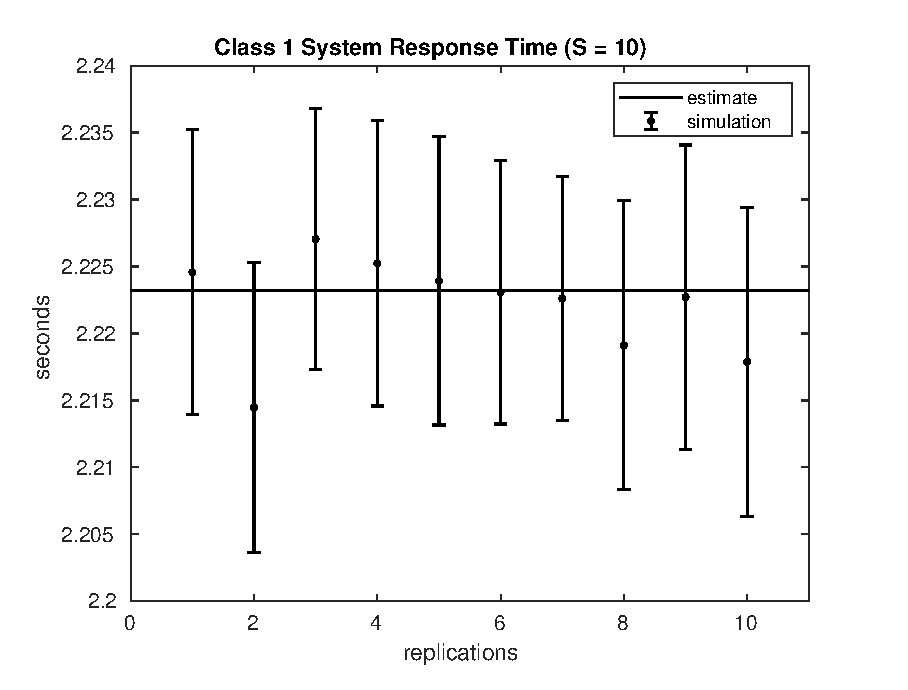
\includegraphics[width=\textwidth]{figures/simul/10_500K_s1}
\caption{classe 1}
\label{10_s1}
\end{subfigure}
%
\begin{subfigure}[t]{0.49\textwidth}
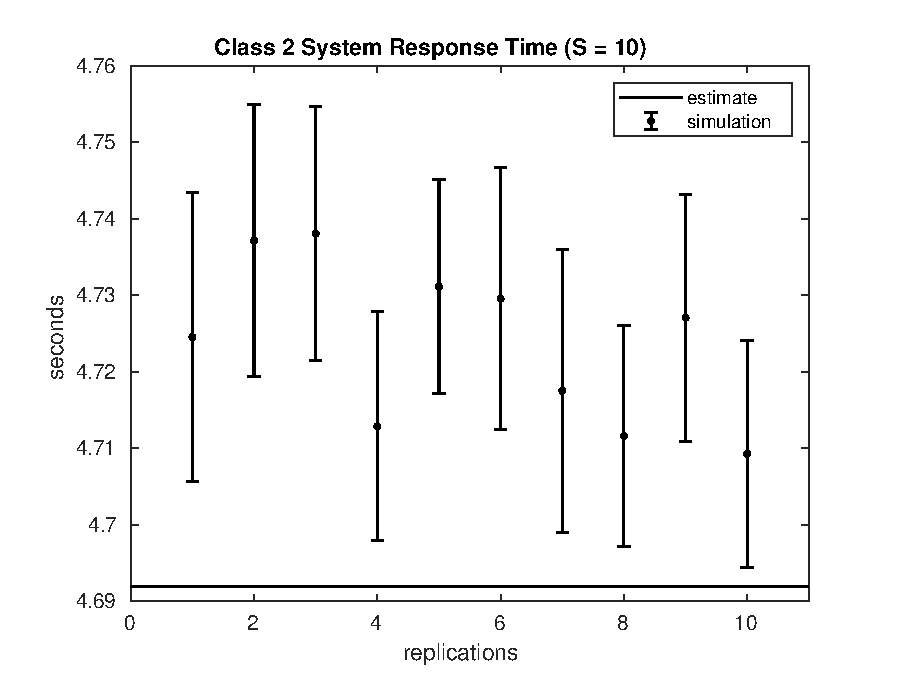
\includegraphics[width=\textwidth]{figures/simul/10_500K_s2}
\caption{classe 2}
\label{10_s2}
\end{subfigure}
%
\begin{subfigure}[t]{0.5\textwidth}
\includegraphics[width=\textwidth]{figures/simul/10_500K_s}
\caption{globale}
\label{10_s}
\end{subfigure}
%
\caption{tempo di risposta medio sistema per $S = 10$}
\end{figure}
%
\begin{table}[!h]
\begin{tabular}{c|r@{.}l|r@{.}l|r@{.}l}
& \multicolumn{2}{|c|}{$S_1$}
& \multicolumn{2}{|c|}{$S_2$}
& \multicolumn{2}{|c}{$S$} 
\\          
\hline
R1      & $2$&$2246 \pm 0.0107$ & $4$&$7245 \pm 0.0188$ & $3$&$7460 \pm 0.0129$ \\
R2      & $2$&$2145 \pm 0.0108$ & $4$&$7371 \pm 0.0178$ & $3$&$7527 \pm 0.0124$ \\
R3      & $2$&$2270 \pm 0.0098$ & $4$&$7381 \pm 0.0166$ & $3$&$7564 \pm 0.0114$ \\
R4      & $2$&$2252 \pm 0.0106$ & $4$&$7129 \pm 0.0150$ & $3$&$7412 \pm 0.0105$ \\
R5      & $2$&$2239 \pm 0.0108$ & $4$&$7311 \pm 0.0139$ & $3$&$7478 \pm 0.0103$ \\
R6      & $2$&$2231 \pm 0.0098$ & $4$&$7295 \pm 0.0171$ & $3$&$7509 \pm 0.0115$ \\
R7      & $2$&$2226 \pm 0.0091$ & $4$&$7175 \pm 0.0185$ & $3$&$7427 \pm 0.0120$ \\
R8      & $2$&$2191 \pm 0.0108$ & $4$&$7116 \pm 0.0144$ & $3$&$7398 \pm 0.0098$ \\
R9      & $2$&$2227 \pm 0.0114$ & $4$&$7271 \pm 0.0161$ & $3$&$7530 \pm 0.0114$ \\
R10     & $2$&$2179 \pm 0.0115$ & $4$&$7093 \pm 0.0148$ & $3$&$7372 \pm 0.0103$ \\
STIMA   & $2$&$2232$            & $4$&$6920$            & $3$&$7286$            \\
MAX ERR & $0$&$0136 \ (0.6\%)$  & $0$&$0629 \ (1.3\%)$  & $0$&$0392 \ (1.0\%)$    
\end{tabular}
\centering
\caption{Confronto tempi di risposta sistema per $S=10$}
\label{tab:10_s}
\end{table}

%%%%%%%%%%%%%%%%%%%%%%%%%%%%%%%%%%%%%%%%%%%%%%%%%%%%%%%%%%%%%%%%%%%%%%%%%%%%%%%%
\subsubsection{Popolazione: Cloudlet}
%
\begin{figure}[!h]
\centering
%
\begin{subfigure}[t]{0.49\textwidth}
\includegraphics[width=\textwidth]{figures/simul/10_500K_n1clet}
\caption{classe 1}
\label{10_n1clet}
\end{subfigure}
%
\begin{subfigure}[t]{0.49\textwidth}
\includegraphics[width=\textwidth]{figures/simul/10_500K_n2clet}
\caption{classe 2}
\label{10_n2clet}
\end{subfigure}
%
\begin{subfigure}[t]{0.5\textwidth}
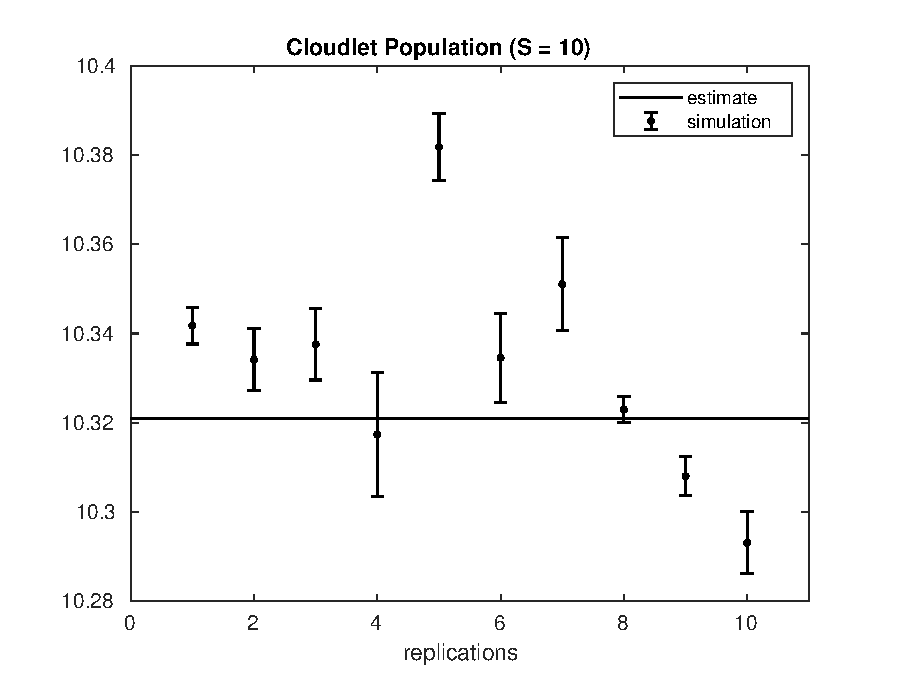
\includegraphics[width=\textwidth]{figures/simul/10_500K_nclet}
\caption{globale}
\label{10_nclet}
\end{subfigure}
%
\caption{popolazione media cloudlet per $S = 10$}
\end{figure}
%
\begin{table}[!h]
\begin{tabular}{c|r@{.}l|r@{.}l|r@{.}l}
& \multicolumn{2}{|c|}{$N_1^{clet}$}
& \multicolumn{2}{|c|}{$N_2^{clet}$}
& \multicolumn{2}{|c}{$N_{clet}$} 
\\          
\hline
R1      & $8$&$9175 \pm 0.0070$ & $1$&$4243 \pm 0.0045$ & $10$&$3418 \pm 0.0041$ \\
R2      & $8$&$8801 \pm 0.0152$ & $1$&$4540 \pm 0.0095$ & $10$&$3341 \pm 0.0070$ \\
R3      & $8$&$9380 \pm 0.0115$ & $1$&$3996 \pm 0.0042$ & $10$&$3376 \pm 0.0080$ \\
R4      & $8$&$8389 \pm 0.0202$ & $1$&$4784 \pm 0.0068$ & $10$&$3174 \pm 0.0138$ \\
R5      & $8$&$9575 \pm 0.0109$ & $1$&$4243 \pm 0.0041$ & $10$&$3817 \pm 0.0074$ \\
R6      & $8$&$8816 \pm 0.0205$ & $1$&$4530 \pm 0.0106$ & $10$&$3346 \pm 0.0099$ \\
R7      & $8$&$9220 \pm 0.0190$ & $1$&$4291 \pm 0.0097$ & $10$&$3510 \pm 0.0104$ \\
R8      & $8$&$8451 \pm 0.0088$ & $1$&$4778 \pm 0.0062$ & $10$&$3229 \pm 0.0029$ \\
R9      & $8$&$8301 \pm 0.0065$ & $1$&$4780 \pm 0.0039$ & $10$&$3081 \pm 0.0043$ \\
R10     & $8$&$8036 \pm 0.0176$ & $1$&$4895 \pm 0.0111$ & $10$&$2931 \pm 0.0069$ \\
STIMA   & $8$&$8841$            & $1$&$4370$            & $10$&$3211$            \\
MAX ERR & $0$&$0842 \ (0.9\%)$  & $0$&$0637 \ (4.3\%)$  & $0$&$0681 \ (0.7\%)$     
\end{tabular}
\centering
\caption{Confronto popolazione cloudlet per $S=10$}
\label{tab:10_nclet}
\end{table}

%%%%%%%%%%%%%%%%%%%%%%%%%%%%%%%%%%%%%%%%%%%%%%%%%%%%%%%%%%%%%%%%%%%%%%%%%%%%%%%%
\subsubsection{Popolazione: Cloud}
%
\begin{figure}[!h]
\centering
%
\begin{subfigure}[t]{0.49\textwidth}
\includegraphics[width=\textwidth]{figures/simul/10_500K_n1cloud}
\caption{classe 1}
\label{10_n1cloud}
\end{subfigure}
%
\begin{subfigure}[t]{0.49\textwidth}
\includegraphics[width=\textwidth]{figures/simul/10_500K_n2cloud}
\caption{classe 2}
\label{10_n2cloud}
\end{subfigure}
%
\begin{subfigure}[t]{0.5\textwidth}
\includegraphics[width=\textwidth]{figures/simul/10_500K_ncloud}
\caption{globale}
\label{10_ncloud}
\end{subfigure}
%
\caption{popolazione media cloud per $S = 10$}
\end{figure}
%
\begin{table}[!h]
\begin{tabular}{c|r@{.}l|r@{.}l|r@{.}l}
& \multicolumn{2}{|c|}{$N_1^{cloud}$}
& \multicolumn{2}{|c|}{$N_2^{cloud}$}
& \multicolumn{2}{|c}{$N_{cloud}$} 
\\          
\hline
R1      & $0$&$0049 \pm 0.0004$ & $26$&$9995 \pm 0.0462$ & $27$&$0044 \pm 0.0464$ \\
R2      & $0$&$0170 \pm 0.0019$ & $26$&$9781 \pm 0.0227$ & $26$&$9951 \pm 0.0224$ \\
R3      & $0$&$0053 \pm 0.0004$ & $27$&$1424 \pm 0.0596$ & $27$&$1477 \pm 0.0597$ \\
R4      & $0$&$0084 \pm 0.0008$ & $26$&$7608 \pm 0.0387$ & $26$&$7691 \pm 0.0394$ \\
R5      & $0$&$0088 \pm 0.0006$ & $26$&$7727 \pm 0.0602$ & $26$&$7815 \pm 0.0598$ \\
R6      & $0$&$0067 \pm 0.0003$ & $27$&$1679 \pm 0.0611$ & $27$&$1746 \pm 0.0613$ \\
R7      & $0$&$0099 \pm 0.0005$ & $27$&$0170 \pm 0.0386$ & $27$&$0269 \pm 0.0389$ \\
R8      & $0$&$0086 \pm 0.0005$ & $26$&$8463 \pm 0.0144$ & $26$&$8549 \pm 0.0143$ \\
R9      & $0$&$0060 \pm 0.0005$ & $27$&$1525 \pm 0.0322$ & $27$&$1585 \pm 0.0321$ \\
R10     & $0$&$0073 \pm 0.0003$ & $26$&$6949 \pm 0.0772$ & $26$&$7022 \pm 0.0772$ \\
STIMA   & $0$&$0086$            & $26$&$6456$            & $26$&$6542$            \\
MAX ERR & $0$&$0103 \ (60.5\%)$ & $0$&$5835 \ (2.1\%)$   & $0$&$5817 \ (2.1\%)$     
\end{tabular}
\centering
\caption{Confronto popolazione cloud per $S=10$}
\label{tab:10_ncloud}
\end{table}

%%%%%%%%%%%%%%%%%%%%%%%%%%%%%%%%%%%%%%%%%%%%%%%%%%%%%%%%%%%%%%%%%%%%%%%%%%%%%%%%
\subsubsection{Popolazione: Sistema}
%
\begin{figure}[!h]
\centering
%
\begin{subfigure}[t]{0.49\textwidth}
\includegraphics[width=\textwidth]{figures/simul/10_500K_n1}
\caption{classe 1}
\label{10_n1}
\end{subfigure}
%
\begin{subfigure}[t]{0.49\textwidth}
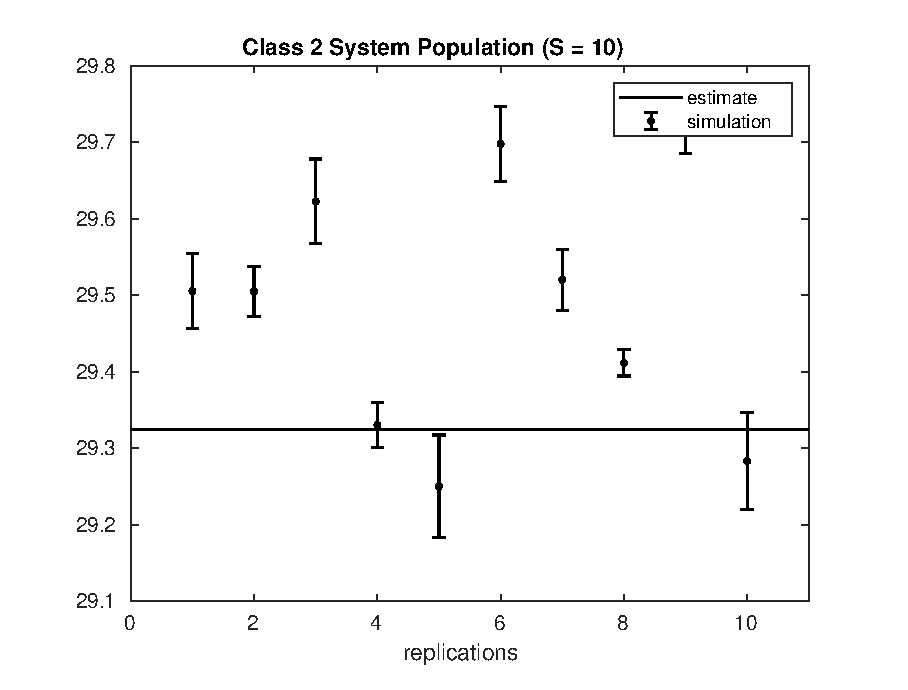
\includegraphics[width=\textwidth]{figures/simul/10_500K_n2}
\caption{classe 2}
\label{10_n2}
\end{subfigure}
%
\begin{subfigure}[t]{0.5\textwidth}
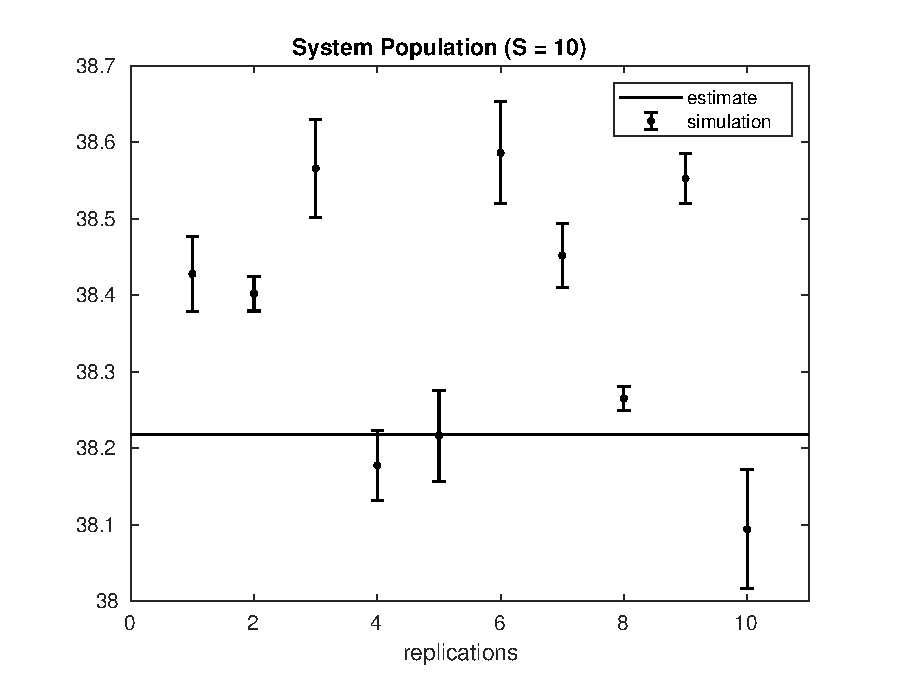
\includegraphics[width=\textwidth]{figures/simul/10_500K_n}
\caption{globale}
\label{10_n}
\end{subfigure}
%
\caption{popolazione media sistema per $S = 10$}
\end{figure}
%
\begin{table}[!h]
\begin{tabular}{c|r@{.}l|r@{.}l|r@{.}l}
& \multicolumn{2}{|c|}{$N_1$}
& \multicolumn{2}{|c|}{$N_2$}
& \multicolumn{2}{|c}{$N$} 
\\          
\hline
R1      & $8$&$9224 \pm 0.0071$ & $29$&$5053 \pm 0.0488$ & $38$&$4277 \pm 0.0492$ \\
R2      & $8$&$8971 \pm 0.0168$ & $29$&$5050 \pm 0.0328$ & $38$&$4021 \pm 0.0228$ \\
R3      & $8$&$9433 \pm 0.0118$ & $29$&$6224 \pm 0.0554$ & $38$&$5658 \pm 0.0642$ \\
R4      & $8$&$8473 \pm 0.0207$ & $29$&$3304 \pm 0.0296$ & $38$&$1777 \pm 0.0459$ \\
R5      & $8$&$9662 \pm 0.0113$ & $29$&$2504 \pm 0.0670$ & $38$&$2166 \pm 0.0594$ \\
R6      & $8$&$8883 \pm 0.0206$ & $29$&$6977 \pm 0.0491$ & $38$&$5859 \pm 0.0665$ \\
R7      & $8$&$9318 \pm 0.0191$ & $29$&$5201 \pm 0.0397$ & $38$&$4519 \pm 0.0418$ \\
R8      & $8$&$8537 \pm 0.0085$ & $29$&$4116 \pm 0.0172$ & $38$&$2653 \pm 0.0160$ \\
R9      & $8$&$8361 \pm 0.0067$ & $29$&$7164 \pm 0.0312$ & $38$&$5525 \pm 0.0329$ \\
R10     & $8$&$8109 \pm 0.0175$ & $29$&$2834 \pm 0.0631$ & $38$&$0943 \pm 0.0779$ \\
STIMA   & $8$&$8927$            & $29$&$3250$            & $38$&$2177$            \\
MAX ERR & $0$&$0848 \ (0.9\%)$  & $0$&$4225 \ (1.4\%)$   & $0$&$4347 \ (1.1\%)$     
\end{tabular}
\centering
\caption{Confronto popolazione sistema per $S=10$}
\label{tab:10_n}
\end{table}

%%%%%%%%%%%%%%%%%%%%%%%%%%%%%%%%%%%%%%%%%%%%%%%%%%%%%%%%%%%%%%%%%%%%%%%%%%%%%%%%
\subsubsection{Throughput: Cloudlet}
%
\begin{figure}[!h]
\centering
%
\begin{subfigure}[t]{0.49\textwidth}
\includegraphics[width=\textwidth]{figures/simul/10_500K_x1clet}
\caption{classe 1}
\label{10_x1clet}
\end{subfigure}
%
\begin{subfigure}[t]{0.49\textwidth}
\includegraphics[width=\textwidth]{figures/simul/10_500K_x2clet}
\caption{classe 2}
\label{10_x2clet}
\end{subfigure}
%
\begin{subfigure}[t]{0.5\textwidth}
\includegraphics[width=\textwidth]{figures/simul/10_500K_xclet}
\caption{globale}
\label{10_xclet}
\end{subfigure}
%
\caption{throughput cloudlet per $S = 10$}
\end{figure}
%
\begin{table}[!h]
\begin{tabular}{c|r@{.}l|r@{.}l|r@{.}l}
& \multicolumn{2}{|c|}{$X_1^{clet}$}
& \multicolumn{2}{|c|}{$X_2^{clet}$}
& \multicolumn{2}{|c}{$X_{clet}$} 
\\          
\hline
R1      & $4$&$0054 \pm 0.0043$ & $0$&$3054 \pm 0.0013$ & $4$&$3108 \pm 0.0047$ \\
R2      & $4$&$0040 \pm 0.0042$ & $0$&$3145 \pm 0.0013$ & $4$&$3185 \pm 0.0030$ \\
R3      & $4$&$0152 \pm 0.0033$ & $0$&$3052 \pm 0.0011$ & $4$&$3204 \pm 0.0030$ \\
R4      & $3$&$9783 \pm 0.0036$ & $0$&$3171 \pm 0.0009$ & $4$&$2954 \pm 0.0033$ \\
R5      & $4$&$0239 \pm 0.0028$ & $0$&$3063 \pm 0.0014$ & $4$&$3302 \pm 0.0032$ \\
R6      & $3$&$9924 \pm 0.0064$ & $0$&$3074 \pm 0.0033$ & $4$&$2997 \pm 0.0043$ \\
R7      & $4$&$0059 \pm 0.0083$ & $0$&$3029 \pm 0.0025$ & $4$&$3089 \pm 0.0064$ \\
R8      & $3$&$9943 \pm 0.0038$ & $0$&$3153 \pm 0.0012$ & $4$&$3096 \pm 0.0041$ \\
R9      & $3$&$9836 \pm 0.0032$ & $0$&$3192 \pm 0.0018$ & $4$&$3028 \pm 0.0041$ \\
R10     & $3$&$9895 \pm 0.0043$ & $0$&$3248 \pm 0.0034$ & $4$&$3143 \pm 0.0022$ \\
STIMA   & $3$&$9978$            & $0$&$3880$            & $4$&$3858$            \\
MAX ERR & $0$&$0288 \ (0.7\%)$  & $0$&$0826 \ (27.3\%)$ & $0$&$0872 \ (2.0\%)$    
\end{tabular}
\centering
\caption{Confronto throughput cloudlet per $S=10$}
\label{tab:10_xclet}
\end{table}

%%%%%%%%%%%%%%%%%%%%%%%%%%%%%%%%%%%%%%%%%%%%%%%%%%%%%%%%%%%%%%%%%%%%%%%%%%%%%%%%
\subsubsection{Throughput: Cloud}
%
\begin{figure}[!h]
\centering
%
\begin{subfigure}[t]{0.49\textwidth}
\includegraphics[width=\textwidth]{figures/simul/10_500K_x1cloud}
\caption{classe 1}
\label{10_x1cloud}
\end{subfigure}
%
\begin{subfigure}[t]{0.49\textwidth}
\includegraphics[width=\textwidth]{figures/simul/10_500K_x2cloud}
\caption{classe 2}
\label{10_x2cloud}
\end{subfigure}
%
\begin{subfigure}[t]{0.5\textwidth}
\includegraphics[width=\textwidth]{figures/simul/10_500K_xcloud}
\caption{globale}
\label{10_xcloud}
\end{subfigure}
%
\caption{throughput cloud per $S = 10$}
\end{figure}
%
\begin{table}[!h]
\begin{tabular}{c|r@{.}l|r@{.}l|r@{.}l}
& \multicolumn{2}{|c|}{$X_1^{cloud}$}
& \multicolumn{2}{|c|}{$X_2^{cloud}$}
& \multicolumn{2}{|c}{$X_{cloud}$} 
\\          
\hline
R1      & $0$&$0013 \pm 0.0001$ & $5$&$9374 \pm 0.0096$ & $5$&$9388 \pm 0.0096$ \\
R2      & $0$&$0035 \pm 0.0003$ & $5$&$9086 \pm 0.0065$ & $5$&$9121 \pm 0.0063$ \\
R3      & $0$&$0015 \pm 0.0001$ & $5$&$9504 \pm 0.0086$ & $5$&$9519 \pm 0.0087$ \\
R4      & $0$&$0020 \pm 0.0001$ & $5$&$9103 \pm 0.0072$ & $5$&$9124 \pm 0.0073$ \\
R5      & $0$&$0021 \pm 0.0001$ & $5$&$8990 \pm 0.0054$ & $5$&$9011 \pm 0.0054$ \\
R6      & $0$&$0019 \pm 0.0001$ & $5$&$9307 \pm 0.0128$ & $5$&$9325 \pm 0.0128$ \\
R7      & $0$&$0025 \pm 0.0001$ & $5$&$9653 \pm 0.0041$ & $5$&$9678 \pm 0.0042$ \\
R8      & $0$&$0024 \pm 0.0001$ & $5$&$9307 \pm 0.0033$ & $5$&$9331 \pm 0.0034$ \\
R9      & $0$&$0016 \pm 0.0001$ & $5$&$9552 \pm 0.0064$ & $5$&$9568 \pm 0.0064$ \\
R10     & $0$&$0021 \pm 0.0001$ & $5$&$9028 \pm 0.0126$ & $5$&$9049 \pm 0.0125$ \\
STIMA   & $0$&$0022$            & $5$&$8620$            & $5$&$8642$            \\
MAX ERR & $0$&$0017 \ (47.3\%)$ & $0$&$1074 \ (1.8\%)$  & $0$&$1078 \ (1.8\%)$    
\end{tabular}
\centering
\caption{Confronto throughput cloud per $S=10$}
\label{tab:10_xcloud}
\end{table}

%%%%%%%%%%%%%%%%%%%%%%%%%%%%%%%%%%%%%%%%%%%%%%%%%%%%%%%%%%%%%%%%%%%%%%%%%%%%%%%%
\subsubsection{Throughput: Sistema}
%
\begin{figure}[!h]
\centering
%
\begin{subfigure}[t]{0.49\textwidth}
\includegraphics[width=\textwidth]{figures/simul/10_500K_x1}
\caption{classe 1}
\label{10_x1}
\end{subfigure}
%
\begin{subfigure}[t]{0.49\textwidth}
\includegraphics[width=\textwidth]{figures/simul/10_500K_x2}
\caption{classe 2}
\label{10_x2}
\end{subfigure}
%
\begin{subfigure}[t]{0.5\textwidth}
\includegraphics[width=\textwidth]{figures/simul/10_500K_x}
\caption{globale}
\label{10_x}
\end{subfigure}
%
\caption{throughput sistema per $S = 10$}
\end{figure}
%
\begin{table}[!h]
\begin{tabular}{c|r@{.}l|r@{.}l|r@{.}l}
& \multicolumn{2}{|c|}{$X_1$}
& \multicolumn{2}{|c|}{$X_2$}
& \multicolumn{2}{|c}{$X$} 
\\          
\hline
R1      & $4$&$0067 \pm 0.0044$ & $6$&$2429 \pm 0.0103$ & $10$&$2496 \pm 0.0140$ \\
R2      & $4$&$0076 \pm 0.0044$ & $6$&$2231 \pm 0.0074$ & $10$&$2306 \pm 0.0060$ \\
R3      & $4$&$0167 \pm 0.0033$ & $6$&$2556 \pm 0.0085$ & $10$&$2723 \pm 0.0108$ \\
R4      & $3$&$9803 \pm 0.0037$ & $6$&$2274 \pm 0.0076$ & $10$&$2077 \pm 0.0096$ \\
R5      & $4$&$0260 \pm 0.0028$ & $6$&$2053 \pm 0.0063$ & $10$&$2313 \pm 0.0069$ \\
R6      & $3$&$9942 \pm 0.0065$ & $6$&$2381 \pm 0.0109$ & $10$&$2323 \pm 0.0168$ \\
R7      & $4$&$0084 \pm 0.0084$ & $6$&$2683 \pm 0.0027$ & $10$&$2766 \pm 0.0097$ \\
R8      & $3$&$9967 \pm 0.0037$ & $6$&$2461 \pm 0.0029$ & $10$&$2428 \pm 0.0037$ \\
R9      & $3$&$9852 \pm 0.0032$ & $6$&$2744 \pm 0.0066$ & $10$&$2596 \pm 0.0090$ \\
R10     & $3$&$9916 \pm 0.0042$ & $6$&$2276 \pm 0.0105$ & $10$&$2192 \pm 0.0121$ \\
STIMA   & $4$&$0000$            & $6$&$2500$            & $10$&$2500$            \\
MAX ERR & $0$&$0288 \ (0.7\%)$  & $0$&$0384 \ (0.6\%)$  & $0$&$0363 \ (0.4\%)$     
\end{tabular}
\centering
\caption{Confronto throughput sistema per $S=10$}
\label{tab:10_x}
\end{table}

%
%
%%%%%%%%%%%%%%%%%%%%%%%%%%%%%%%%%%%%%%%%%%%%%%%%%%%%%%%%%%%%%%%%%%%%%%%%%%%%%%%%
%%%%%%%%%%%%%%%%%%%%%%%%%%%%%%%%%%%%%%%%%%%%%%%%%%%%%%%%%%%%%%%%%%%%%%%%%%%%%%%%
\subsection{Scenario 3: $\mathbf{S=\frac{3}{4}N=15}$}
%
%
%%%%%%%%%%%%%%%%%%%%%%%%%%%%%%%%%%%%%%%%%%%%%%%%%%%%%%%%%%%%%%%%%%%%%%%%%%%%%%%%
%%%%%%%%%%%%%%%%%%%%%%%%%%%%%%%%%%%%%%%%%%%%%%%%%%%%%%%%%%%%%%%%%%%%%%%%%%%%%%%%
\subsection{Scenario 4: $\mathbf{S=\frac{N}{4}=5}$}
